\chapter{Related Work}\label{ch:related-work}
This chapter provides a comprehensive overview of the preceding works that are related to the subject of this thesis. This chapter first presents the use cases of different \ac{ml} algorithms in the field of power grids and its operation. Secondly, a series of past works will be presented, providing both general and power grid-specific benchmarks for \ac{rl} algorithms.


% ============================================================
% ============================================================
\section{Applications on Power Grids}\label{sec:application-power-grids}
This section is focused on past work on the application of \ac{ml} algorithms on power grids. Firstly, a number of examples will be given of forecasting systems, which provide estimates of future states of grid components. Subsequently, an analysis of a range of \ac{rl} algorithms that control power grids with different objectives will be made. The following summary will demonstrate how past works have already demonstrated the usefulness of \ac{rl} agent-based control systems in managing grids, and how they are used in a variety of situations, from the control of specific grid components to the alteration of the grid's topology in order to optimise power flow. 


% ++++++++++++++++++++++++++++++++++++++++++++++++++++++++++++
\subsection{Forecasting Systems}
Supervised learning approaches are useful for forecasting systems in power grids. Most of these systems solve a time-series problem, meaning the data is time-dependent. These systems are trained to predict specific labels in the grid at future timestamps, which helps maintain grid stability. 
Studies such as \citet{shortTermLoadForecasting} and \citet{loadForecastingDeepNN} demonstrate how short-term load forecasting is achieved using supervised learning. This is useful for cost estimation for power grid customers, or for predicting energy needs in order to plan when to generate more or less power.

Regarding generators, works such as \citet{meka2021robust} demonstrate how a model that forecasts wind generation is trained using meteorological data together with wind power production. This helps manage the variability caused by wind generation, as with other renewable energies, and makes it easier to integrate wind energy into power grids. 

Regarding the entire power grid, the work of \citet{ngo2024physics} focuses on the implementation of a GNN, which estimates the state of power grid components. This paper presents a common representation of power grids as graphs, where the nodes represent buses and the edges represent transmission lines. This representation is evident in other frameworks and simulation environments, which will be discussed in later sections. Supervised learning is used to train and estimate bus voltage magnitudes, voltage phase angles, and other power grid states using grid measurements.


% ++++++++++++++++++++++++++++++++++++++++++++++++++++++++++++ 
\subsection{Grid Control Systems}\label{ssec:grid-ctrl-systems}
\ac{rl} has use cases in grid control, since power grid operation involves decision-making that needs to be optimised. The \ac{rl} agent performs sequential control decisions while improving its policy to achieve a more stable grid and optimal resource usage. 
Using \ac{rl} for this problem has become more important as the proportion of renewable energy in power grids has increased, as previously mentioned, and these sources have a more unpredictable power generation pattern. Improvements in \ac{rl} and \ac{drl} now enable agents to solve complex problems involving large data sets \cite{glavic2017reinforcement}. Due to this progress, more researchers have attempted to use \ac{rl} for power grid operation \cite{fan2022powergym}.

The typical actions in power grid operation can be divided into three categories. \textbf{Control actions} manage the adjustable components of the power grid. For example, dispatch actions control power generation by increasing or decreasing the output of power plants to match the current load demand. Another example is voltage control throughout the grid. \textbf{Topology actions} modify the grid's configuration, e.g. by opening or closing transmission lines, changing the busbar to which a line is connected, or splitting or merging substations. These actions are useful for controlling power flow in the grid and for avoiding or handling congestion (overloaded transmission lines). The final type of action is \textbf{protection} or \textbf{emergency action}. These actions prevent cascading failures and attempt to restore the grid to a safe state. Examples include load shedding, which disconnects part of the loads from the power grid to temporarily reduce the power demand for the grid, generator tripping, which disconnects generators from the grid to protect them \cite{protecting_synchronous_generators}, or emergency switching, which changes the network's topology to prevent cascading failures throughout the grid components.

\subsubsection{Control Actions on Power Grids}
The work of \citet{glavic2017reinforcement} shows how \ac{rl} has already been used in past research for grid control or emergency actions. Figure \ref{fig:rl-framework-powergrid} shows a framework for building a \ac{rl} algorithm that makes decisions over a power grid, as mentioned in the work. The research mentioned in this paper has considered \ac{rl} agents for a variety of use cases, such as making market decisions through electricity market simulations and controlling the grid, including voltage control, automatic generation control, power demand control, and system restoration to bring the power grid back to a stable state. This work demonstrates how \ac{rl} is already considered an effective approach to solving a variety of control and decision problems in power grids.

\begin{figure}[htp] 
    \centering
    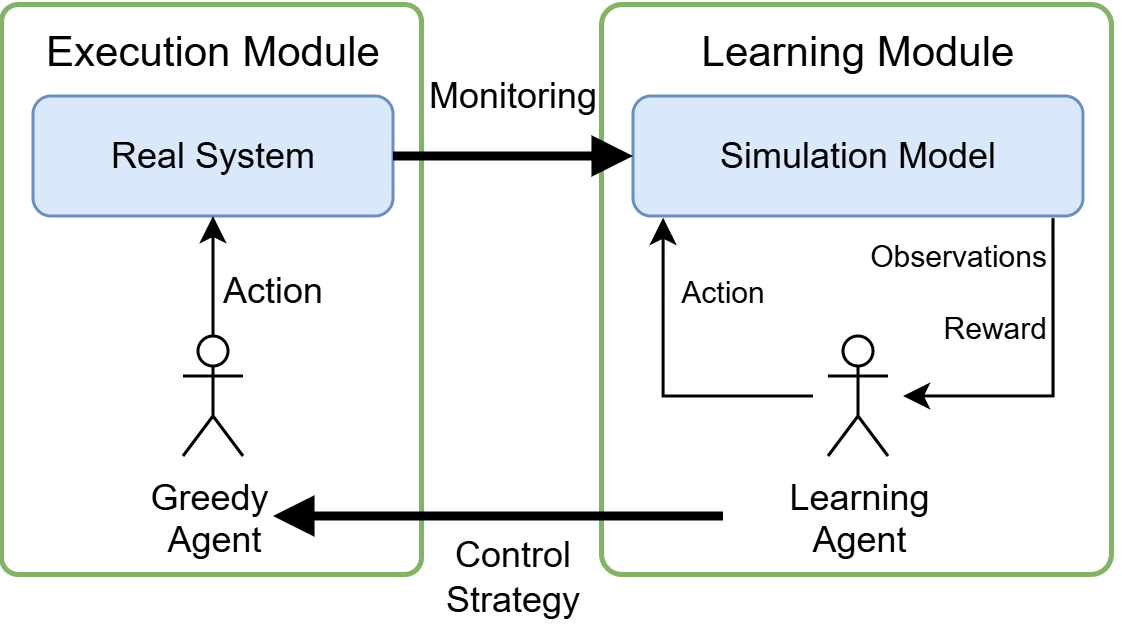
\includegraphics[width=0.8\textwidth]{images/related_work/RL_framework_glavic.png}
    \caption{Framework for a \ac{rl} algorithm in power grid decision and control}
    \label{fig:rl-framework-powergrid}
\end{figure}

Another grid control approach is presented in \citet{barg2023deep}, which uses \ac{drl} to regulate voltage levels at all buses to ensure reliable operation. Each state in the \ac{rl} algorithm contains information on the bus voltages, power flows and network conditions. The agent's actions use controllable grid components to regulate voltage levels. The agent is rewarded for keeping voltages within limits, reducing voltage violations and avoiding unnecessary control actions \cite{barg2023deep}.


\subsubsection{Topology Actions on Power Grids}
A considerable amount of research has been conducted on topology actions involving \ac{rl}. One important research project in this area is the \ac{l2rpn} challenge. The aim of this challenge is to design agents that operate safely over power grids. 
To run the agents for the challenge, the \textbf{Grid2Op} framework was developed. This section refers to the paper by \citet{l2rpn} for details of \ac{l2rpn} and to the Grid2Op documentation to summarise Grid2Op.

Grid2Op emulates the behaviour of a power grid, exposing agents to maintenance operations and topology changes within the grid. The framework focuses on \ac{rl} development and enables actions such as connecting or disconnecting transmission lines, moving grid components (e.g. lines, generators, and loads) to another busbar, redispatching generators, curtailing renewable generators (i.e. asking them to produce less than they are capable of), and controlling power storage units. Grid simulations commonly use \textbf{pandapower}, an open-source library for power system modelling and analysis. This tool enables the simulation of \ac{ac} and \ac{dc} power flow, the execution of \ac{opf}, and the analysis of network states over time \cite{pandapower}.

The paper by \citet{l2rpn} presents the results of the \ac{l2rpn} challenge. For this, an industry-standard synthetic network was used, and the agents had to comply with a few constraints. Deterministic events, such as maintenance, and stochastic events, such as targeted attacks by an adversarial opponent, can disconnect power lines for several hours. Additionally, if a line is overloaded for too long, it automatically disconnects, which can lead to cascading failures. The agent must wait before using these lines again, as it takes a few hours for them to be reconnected. Furthermore, to prevent the overuse or failure of expensive network components, the agent is not permitted to act on the same component too frequently. The agent's run is terminated by a "Game Over" condition when the total demand is not met. In the \ac{l2rpn} challenge, only two actions are permitted: topology changes and changes to the power generation of the power plants within the grid. Each action is checked against the previously mentioned constraints before being fed into a power flow simulator to calculate the next network state.

Each of the participants' agents went through 24 test scenarios. For each scenario, the participants were given a validation dataset during training and a test dataset for the final leaderboard. The evaluation and scoring of each agent are discussed in detail in Section \ref{ssec:power-benchmark}. 
Of the approaches, the three best ones all used \ac{rl} to solve this optimisation problem. 
The agent with the best performance reduced the possible actions to 1000 to reduce complexity. They used a policy parameterised by a neural network with a few million parameters, which they trained with an evolutionary algorithm instead of standard \ac{drl} strategies (e.g. \ac{ppo} or \ac{dqn}). In the evolutionary algorithm, multiple policies were trained and the best ones were selected and mutated, iteratively improving the policy weights. 
The second-best agent initially used expert-guided exploration to reduce the action space to 200 actions. They then trained a neural network to imitate this expert agent, although this imitation agent performed slightly worse. Finally, they used an actor-critic model with \ac{ppo}, initialised with the imitation agent and trained to improve long-term planning. This improved their strategy, earning them second place in the challenge. The third-best-performing agent used a \ac{dqn} variation that directly learns a policy mapping grid states to topology actions.

This challenge encouraged many participants to develop different approaches to solving the problem of power grid operation. The Grid2Op framework made it possible for many developers and researchers to begin researching agents in the power grid domain. The resulting agents demonstrated robustness in challenging grid scenarios, successfully handling long action sequences even under strong perturbations. Notably, agents showed the potential to augment knowledge of grid flexibility beyond human capability, which would already be valuable for grid operators. This suggests that \ac{ml} algorithms, particularly \ac{rl}-based approaches, hold promise as tools to support \acp{tso} in grid operation.

Similar to Grid2Op, the work by \citet{pptopogym} presents \textbf{PPTopoGym}, a lightweight topology optimisation environment that uses the pandapower library for data structures and power flow calculations. Furthermore, it offers the computation of $N-1$ power flow to test how stable the power grid remains if one line is removed. This feature is not included in the \ac{l2rpn} competitions, as mentioned in Section \ref{ssec:power-benchmark}. The PPTopoGym environment supports topology actions such as substation reconfiguration, as well as line, switch and transformer switching \cite{pptopogym}.

Another survey discussing topology actions in power grids is done by \citet{grl4powergrids}. It focuses on \ac{gnn} and how to use them in \ac{grl}. Since power grids can be naturally modelled as graphs, \acp{gnn} combined with \ac{rl} are suitable for this optimisation problem. \acp{gnn} have the functionalities required for feature extraction in graph-structured data, helping \ac{rl} agents to understand complex relationships within grids and make better decisions. The survey presents approaches to \ac{grl} used in topology actions across power grids. In these approaches, the grid state is modelled as a graph from which a \ac{gnn} extracts features. Grid states contain grid topology information, such as bus, generation and load connections, as well as voltages and power flows in transmission lines. The agent's rewards are calculated based on these power flows, the extent to which grid congestion is mitigated, and the level of operational cost reduction.



% ============================================================
% ============================================================
\section{Benchmarking}\label{sec:rw-benchmarking}
This section presents previous benchmarking studies in the field of \ac{rl}. It summarises the structure of different benchmarks, using the principles outlined in Section \ref{ssec:principles-benchmark} to evaluate each benchmark's design.


% ++++++++++++++++++++++++++++++++++++++++++++++++++++++++++++
\subsection{Reinforcement Learning Benchmarking}
An established standard for training and testing \ac{rl} agents is \textbf{OpenAI Gym} \cite{gymnasium}. The paper by \citet{gymnasium} showcases the features of this toolkit, which standardises the development and evaluation of \ac{rl} algorithms. OpenAI Gym provides a variety of environments, including control problems, Atari games, and robotics environments. Each agent is evaluated based on its episodic cumulative reward (return) achieved in the test environments, and there used to be a website with a scoreboard where researchers and developers could reproduce or compare other approaches by examining their source code. After OpenAI Gym was no longer maintained, \textbf{Gymnasium} became its successor. The paper by \citet{gymnasium} demonstrates how Gymnasium, just like OpenAI Gym, has become a popular toolkit with millions of downloads since its release. Like OpenAI Gym, Gymnasium contains a standardised environment interface and has built-in environments. Additionally, it has a large ecosystem of external environments, and it is possible to use it with various training libraries (e.g. Stable Baselines 3, CleanRL and Ray RLlib). Like OpenAI Gym, Gymnasium does not benchmark agents directly, but instead offers standardised environments for testing agents. According to the benchmark structure defined in Section \ref{ssec:structure-benchmark}, it contains the data and tasks required for a benchmark evaluation. However, it lacks the metrics and scoring system necessary to provide measurable feedback to agents.

A similar benchmark is the \textbf{Procgen} Benchmark mentioned in \citet{procgen}. Furthermore, it offers a variety of game-like environments. For each environment, a unique scenario is created using procedural generation. This benchmark measures sample efficiency, i.e. how effectively an agent learns from a limited number of experiences or interactions with its environment. Additionally, it measures generalisation, which is an agent's ability to perform well on new, unseen tasks. The procedural generation used in this benchmark is useful to control whether an agent has problems with overfitting to one specific scenario. This makes the benchmark representative by covering diverse scenarios and benchmarking edge cases procedurally. A final single score is calculated based on a mean normalised return value. As it only focuses on two tasks of an \ac{rl} agent, sample efficiency and generalisation, this benchmark is a macro-benchmark. However, when compared to other agents, this benchmark lacks information, as an aggregated score does not show the strengths and weaknesses of the agents, only their overall performance.


% ++++++++++++++++++++++++++++++++++++++++++++++++++++++++++++
\subsection{Benchmarking on Power Grids}\label{ssec:power-benchmark}
There is already past work on benchmarking \ac{rl} agents in power grids, some of which is strongly related to this work. Many of these existing tools use the IEEE test cases presented in \citet{matpower}. These are standardised power grid models offering different grids. For example, IEEE 30-bus, also known as case 30, consists of 30 buses, five generators and 41 lines \cite{matpower}. These models provide realistic grids of various sizes and levels of complexity, making them well-suited to accurately representing real-world scenarios in benchmarks. This section presents the benchmarks that utilise these test cases, and their design will be analysed. 

\subsubsection{PowerGym}
The \textbf{PowerGym} project, introduced in \citet{fan2022powergym}, benchmarks Volt-Var control systems in distribution grids. This means that agents must control voltage (Volt) and reactive power (Var) in order to minimise power losses and voltage violations within the grid. The components used to achieve this are voltage regulators, switchable capacitors, and controllable batteries. The capacitors regulate reactive power, while the batteries regulate active power.
An OpenAI Gym interface is used for the benchmark, making it easier to use with existing \ac{rl} algorithms. The \textbf{OpenDSS} simulator is used for the physical power flow and the test environments are based on IEEE benchmark systems. The benchmarking system is designed solely to compare multiple approaches with each other in the same standardised Volt-Var control environment, where performance is measured using cumulative reward. This reward system penalises voltage violations, power losses, and frequent changes that wear out control devices. It is possible to modify the test environments to increase difficulty, e.g. by scaling the loads, which results in higher power consumption and makes grid stability more difficult.

As for the benchmark design, this work aligns with most of the principles. The objective is clear, as the Volt-Var control target task is specified throughout. Furthermore, it offers a standardised evaluation setup with fixed systems and a uniform structure, which provides reproducible results. As it is possible to evaluate different agents in the same environments, with the same system definitions and reward functions, PowerGym enables direct comparison of agents. Additionally, the paper provides a clear explanation of how the benchmark works and what it evaluates. Lastly, the benchmark is relevant to the application domain as it uses OpenDSS and diverse IEEE test scenarios for simulation, providing sufficient coverage of Volt-Var control scenarios. However, some principles are lacking, such as the fact that the benchmark only provides one cumulative reward score, which might hide the strengths and weaknesses of an agent. Moreover, the environments used in the benchmark only cover four systems, which may not represent every edge case or common scenario. A more diverse selection of scenarios allows for a more in-depth evaluation of agents.

\subsubsection{L2RPN}\label{sssec:l2rpn}
As mentioned in Section \ref{ssec:grid-ctrl-systems}, \ac{l2rpn} is a competition-style benchmark built using the Grid2Op simulation framework. Benchmarking is performed through the \ac{l2rpn} challenge, in which each participant must complete 24 test scenarios. For each scenario, participants were provided with a validation dataset during training and a test dataset for the final leaderboard, with submitted code executed by an evaluation server. Each scenario received a normalised score ranging from -100 to 100, based on the cumulative network operational cost. A score of -100 was given if an immediate blackout occurred, and a score over 0 required the agent to perform better than a do-nothing agent (i.e. an agent that does not interact with the environment). If the scenario was completed without terminating early with a "Game Over", the agent received a score of 80. To achieve the maximum score of 100, the agent's operational cost must be 20\% lower than that of a baseline agent. The leaderboard was created by taking the sum of all the scores from the 24 scenarios.

As for the benchmark principles, this challenge followed most of them. \ac{l2rpn} had a clear objective in ranking the agents by having two sub-objectives, robustness and adaptability. For the adaptability, the agent's ability to handle unseen data distribution of renewable energy mixes is tested. Additionally, due to the fixed evaluation structure of the challenge, reproducibility was ensured, with a standardised evaluation server testing the submitted agents. As all the agents underwent the same process and a fixed set of scenarios and evaluation systems, it was possible to compare multiple agents and thus create a leaderboard ranking. This challenge involved comparing multiple scenarios, showing how each agent performed in different situations. This is important, as benchmarks should show not only the best agent overall, but also its strengths and weaknesses in different situations. Furthermore, the transparent structure of the challenge made the benchmarking process clear. However, the score calculation is not transparent. For example, the difference in robustness between the two best agents, with scores of 59 and 46, is not very intuitive. It is unclear how the calculations work between the fixed score points of -100, 0, 80 and 100. Nevertheless, the benchmark is relevant to the field as the agents operate on a network derived from the IEEE 118-bus system, and the scenarios are realistic, including maintenance events and thermal constraints on assets. Grid2Op's physical simulation of power grids produces realistic grid behaviour. This enables the agents to address real operational issues, such as cascading failures, uncertainty from renewable energy, and reacting to contingencies. Furthermore, the scenarios present diverse problems that \acp{tso} also have to deal with, such as high load or high renewable generation. However, only one core grid environment is used for testing, rather than multiple different topologies, which would create even more diverse scenarios with different grids.


\subsubsection{RL2Grid}
The RL2Grid framework was developed following the work of the \ac{l2rpn} challenge. The work of \citet{rl2grid} presents the framework and its structure. The main goal of RL2Grid is to provide a standardised evaluation of \ac{rl} agents in grid control problems. Previous work showed that researchers used different methods to create their agents, such as custom inputs and reduced action spaces, which made direct comparison difficult. 

RL2Grid uses more grid environments, including seven different power grid systems from Grid2Op, as well as \textbf{ChroniX2Grid} for profiles (i.e. time series descriptions of load demand and power generation), which provides synthetic yet operationally realistic timesteps for the environments. The seven base grids vary in size, ranging from 14 to 118 substations, and each employs a double bus system, meaning the substations have two busbars and each grid component can be connected to one of the two. The grids support features from \ac{l2rpn}, like scheduled line maintenance and random line disconnections caused by an opponent.

Another design change is the addition of two expert-informed heuristics that emulate human operator behaviour and suppress agent actions when the grid is stable. The agent only acts when there is a risk, such as line overloads. However, when the grid is stable enough, the heuristic will incrementally restore the original topology. This reduces the task for the agent to the important parts, improving learning and the agent's sample efficiency. 

Additionally, RL2Grid introduces the concept of \ac{cmdp} to formulate grid safety constraints. In this framework, two key constraint classes arise, one for \ac{lsi} and the other for \ac{tlo}, both of which trigger a higher cost. \ac{lsi} happens when part of the electricity demand cannot be supplied anymore, leading to the disconnection of loads (load shedding), or when the grid splits into separate parts instead of remaining fully connected (islanding). \ac{tlo} occurs when the thermal limits of transmission lines are exceeded or they become disconnected.
The possible actions of each agent are categorised into two classes, either topology control, which involves modifying the topology of substations by disconnecting or reconnecting lines or changing the bus to which a component is connected, or redispatching and curtailment, which involves adjusting power generation. 

The framework has multiple metrics to benchmark agents for the evaluation. The main criterion is survival, defined as how long an agent is able to keep a grid running before terminal failure occurs. To achieve the highest score, an agent must keep the grid running under stable conditions for one episode, consisting of one month of data divided into five-minute steps. 
Furthermore, there are three operational metrics for evaluation, which are line margin, overloads, and topology changes. Line margin defines the remaining spare capacity of the transmission lines, the overloads metric measures the extent to which the agent allows the grid to operate in an overloaded state, and the topology metric defines the extent to which the agent reconfigures the grid relative to the initial grid topology.

RL2Grid has a strong overall benchmark design, especially compared to its predecessor, \ac{l2rpn}. Building on previous work, RL2Grid has a clear objective definition, which is reflected in its components. 
However, reproducibility is only partially guaranteed, as the benchmark contains random components. For example, episodes may start from a randomly sampled time index, and some environments may experience random line disconnections. The rest of the benchmark has fixed definitions, tasks and evaluations, but these random components make it less reproducible and affect comparability, making it partially reliable. However, introducing three operational metrics alongside the survival score makes it easier to identify the strengths and weaknesses of each agent. This improves interpretability, as the operational metrics may explain the survival score result. Furthermore, the paper explains the entire benchmark setup, providing transparency on how each agent is evaluated. 
This benchmark is highly relevant to the field as it features realistic grid simulations with Grid2Op, realistic synthetic grid environments, and constraints and rewards that reflect real \ac{tso} priorities. As the authors mentioned, improvements to realism and relevance could include using real or more realistic synthetic data, and grids on a larger scale. However, this benchmark lacks $N-1$ security, better storage modelling, and other operational details. 
Although RL2Grid has a greater diversity than \ac{l2rpn} with its seven base grids, the number of environments is still limited and may not cover edge cases or test the generalisation of an agent. Much more data or procedural data generation is necessary. 


\subsubsection{Summary of Power Grid Benchmarks}
Table \ref{tab:power-grid-benchmarks} summarises the three power grid benchmarks discussed in this chapter. It compares the benchmarks' task focus, simulation basis, grid diversity, scoring approach, safety handling and reproducibility. While each benchmark advances the field in its own way, all three have limitations in common. The restricted number of grid topologies limits their ability to test generalisation and cover edge cases. Furthermore, the lack of diagnostic tools for analysing results, combined with the largely one-dimensional scoring that most benchmarks rely on, makes it difficult to gain a deeper understanding of an agent's strengths, weaknesses and behaviour.

\begin{table}[htp]
    \centering
    \caption{Comparison of existing \ac{rl} benchmarking tools for power grid operation.}
    \label{tab:power-grid-benchmarks}
    \small
    \renewcommand{\arraystretch}{1.1}
    \begin{tabularx}{\textwidth}{@{}l>{\raggedright\arraybackslash}X>{\raggedright\arraybackslash}X>{\raggedright\arraybackslash}X@{}}
        \toprule
        & \textbf{PowerGym} & \textbf{L2RPN} & \textbf{RL2Grid} \\
        \midrule
        \textbf{Task focus} & Volt-Var control (voltage \& reactive power) & Topology \& redispatch control & Topology \& redispatch control \\ \midrule
        \textbf{Simulator} & OpenDSS & Grid2Op & Grid2Op + ChroniX2Grid \\ \midrule
        \textbf{Grid diversity} & 4 IEEE distribution systems & 1 core grid (IEEE 118-bus derived) & 7 base grids (14--118 substations) \\ \midrule
        \textbf{Scoring} & Single cumulative reward & Normalised score ($-100$ to $100$) per scenario, summed for leaderboard & Survival score + 3 operational metrics (line margin, overloads, topology changes) \\ \midrule
        \textbf{Safety handling} & Penalised in reward (voltage violations) & Game-over on blackout & \ac{cmdp} constraints (load shedding, islanding, thermal limits) \\ \midrule
        \textbf{Reproducibility} & Fully deterministic scenarios & Fixed evaluation server \& scenarios & Partially stochastic (random start indices, random line disconnections) \\
        \bottomrule
    \end{tabularx}
\end{table}